\documentclass[english]{upeeei}
\usepackage[latin9]{inputenc}
\setcounter{secnumdepth}{3}
\setcounter{tocdepth}{3}
\usepackage[active]{srcltx}
\usepackage{units}
\usepackage{parskip}
\usepackage{graphicx}
\usepackage{subfigure} 
\usepackage{url}  
%\usepackage{stfloats}  
\usepackage{amsmath}   
\usepackage{array}
\usepackage{caption}
\usepackage{afterpage}
\usepackage{textcomp}
\usepackage{lscape}
\usepackage{stfloats}
\usepackage{hyphenat}
\usepackage{makeidx}
\usepackage{amssymb}
%\usepackage{underscore}
\fnbelowfloat
\usepackage{times}
\usepackage{multirow}
%\usepackage{float}
\usepackage{circuitikz}
\usepackage[backend=bibtex,bibstyle=ieee,citestyle=numeric-comp]{biblatex}
\addbibresource{Proposal_Part1.bib}
\usepackage{pgfplots}
%%% LyX 2.3.2-2 created this file.  For more info, see http://www.lyx.org/.
%% Do not edit unless you really know what you are doing.
\documentclass[english]{article}
\usepackage[T1]{fontenc}
\usepackage[latin9]{luainputenc}
\usepackage[a4paper]{geometry}
\geometry{verbose,tmargin=0.5in,bmargin=1in,lmargin=0.5in,rmargin=0.5in}
\usepackage{graphicx}

\makeatletter

%%%%%%%%%%%%%%%%%%%%%%%%%%%%%% LyX specific LaTeX commands.
%% Because html converters don't know tabularnewline
\providecommand{\tabularnewline}{\\}

%%%%%%%%%%%%%%%%%%%%%%%%%%%%%% User specified LaTeX commands.
\usepackage{multirow} 
\pagestyle{empty}

\makeatother

\usepackage{babel}
\begin{document}
\noindent \begin{center}
\begin{tabular}{c}

\includegraphics[width=0.625in]{UP_logo_maroon}\tabularnewline
UNIVERSITY OF THE PHILIPPINES\tabularnewline
\end{tabular}
\par\end{center}

\vspace*{\fill}

\begin{center}
    Design of a Raspberry Pi Based Flight Controller for Multirotor Unmanned Aerial Vehicles
\par\end{center}

\vspace*{\fill}

\begin{center}
Louie Isaniel Cachola Henson\\
\par\end{center}

\begin{center}
B.S. Computer Engineering
\par\end{center}

\vspace*{\fill}

\begin{center}
Undergraduate Project Adviser:\\
\par\end{center}

\begin{center}
Charleston Dale Ambatali, MEE \\
Roxanne P. De Leon, ECE, MTM
\par\end{center}

\begin{center}
Electrical and Electronics Engineering Institute 
\par\end{center}

\begin{center}
University of the Philippines Diliman
\par\end{center}

\vspace*{\fill}

\begin{center}
Undergraduate Project Reader:\\
\par\end{center}

\begin{center}
Jhoanna Rhodette I. Pedrasa, PhD
\par\end{center}

\begin{center}
Electrical and Electronics Engineering Institute 
\par\end{center}

\begin{center}
University of the Philippines Diliman
\par\end{center}

\vspace*{\fill}

\begin{center}
Date of Submission 
\par\end{center}

\begin{center}
July 15, 2021
\par\end{center}

\vspace*{\fill}

\begin{center}
Permission is given for the following people to have access to this
thesis: 
\par\end{center}

\noindent \begin{center}
\begin{tabular}{|l|c|}
\cline{1-1} 
Circle one or more concerns: \hspace*{1cm}I\qquad{}P\qquad{} C & \multicolumn{1}{c}{}\tabularnewline
\hline 
Available to the general public & Yes/No\tabularnewline
\hline 
Available only after consultation with author/thesis adviser & Yes/No\tabularnewline
\hline 
Available only to those bound by confidentiality agreement & Yes/No\tabularnewline
\hline 
\multicolumn{1}{l}{\hspace*{10cm}} & \multicolumn{1}{c}{\hspace*{2cm}}\tabularnewline
\end{tabular}
\par\end{center}

Students\textquoteright{} signature/s: \\

Signature/s of undergraduate project advisers: \\

\end{document}

%\includeonly{}
%\usepackage{arydshln}
\pgfplotsset{width=7cm,compat=1.5.1}
\renewcommand*{\bibfont}{\small}

\newcolumntype{L}[1]{>{\raggedright\let\newline\\\arraybackslash\hspace{0pt}}m{#1}}
\newcolumntype{C}[1]{>{\centering\let\newline\\\arraybackslash\hspace{0pt}}m{#1}}
\newcolumntype{R}[1]{>{\raggedleft\let\newline\\\arraybackslash\hspace{0pt}}m{#1}}

\newcommand\ddfrac[2]{\frac{\displaystyle #1}{\displaystyle #2}}
\pgfplotsset{compat=1.14}

\makeatletter

%%%%%%%%%%%%%%%%%%%%%%%%%%%%%% LyX specific LaTeX commands.
\providecommand{\LyX}{L\kern-.1667em\lower.25em\hbox{Y}\kern-.125emX\@}
%% Because html converters don't know tabularnewline
\providecommand{\tabularnewline}{\\}

\@ifundefined{showcaptionsetup}{}{%
 \PassOptionsToPackage{caption=false}{subfig}}
\usepackage{subfig}
\makeatother

\usepackage{babel}

\begin{document}
%%% UP EEEI undergraduate project template
%% v0.1 by Louis P. Alarcon 11/22/2011
%%
%% LyX template - use with the following files:
%% 	uct10_new.clo, uct11_new.clo, uct12_new.clo, upeeei.cls, upeeei.layout
%%
%% Place project title here

\title{Design of a Raspberry Pi Based Flight Controller for Multirotor Unmanned Aerial Vehicles} 

%%
%% Author information

\author{
%% Use \vspace to separate each member
%% Put your names here in alphabetical order
\\Louie Isaniel Cachola Henson \\ 2014-30227 \\ \emph{B.S. Computer Engineering}
}

%%
%% Month and year of submission/graduation
\degreeyear{2021} 
\degreesemester{January} 

% Put your advisers here:
\chair{Charleston Dale Ambatali, MEE 
\\
Roxanne P. De Leon, ECE, MTM
} 
%\othermembers{John Richard Ereso Hizon\\ 
%Joel Joseph Sarco Marciano, Jr.} 
\numberofmembers{1} 

\field{Electrical/Computer/Electronics and Communications Engineering} 
\campus{Diliman} 

\maketitle

% \approvalpage 
% \copyrightpage 
\begin{abstract} 

%Your abstract goes here...


Multirotor unmanned aerial vehicles (or drones) are quick and versatile, often 
proving to be a great asset for various purposes. It is because of this that drones have been integrated into
more industries and fields of study. This necessitates the development of flight controllers that are
cost-effective, versatile and easy to develop. Meanwhile, the Raspberry Pi has shown steady development, quickly
growing more powerful and versatile with each model released. It allows for rapid prototyping while remaining
small and relatively inexpensive, making it a good fit to be a flight controller. Despite this, there are no
publicly available open source flight controllers that are based solely on the Raspberry Pi.
The goal of this project is to develop a flight controller that is readily compatible with the Raspberry Pi, 
thereby taking advantage of the Raspberry Pi's versatility and low cost. Through the use of a modular framework
for the software and the implementation of previously established control algorithms, the project was able to prove
that the development of a Raspberry Pi based flight controller is feasible and could possibly serve as an out-of-the-box
cornerstone for future developments in UAV technology.This is in line with the Advanced 
Defense and Aerospace Materials (ADAM) R\&D's Project Diosa, where the goal is to develop a multirotor UAV using 
low cost materials.


\end{abstract}

\begin{frontmatter}
\setlength{\parskip}{0pt}
\tableofcontents
%\listoftables
\listoffigures
\end{frontmatter}
\def\MASTERDOC{true}

\chapter{Introduction}
Unmanned aerial vehicles (UAVs) continue to be integrated into increasingly diverse environments and
fields. From photography and cinematography, all the way to military applications and even disaster risk reduction and 
management. They are especially useful for reducing the amount of risk that personnel experience by flying to places that 
pose a significant hazard to personnel \cite{ICNSC2010}. Advanced Defense and Aerospace Materials (ADAM) R\&D's Project
Diosa aims to develop a functional but low cost multirotor unmanned aerial vehicle (UAV) for use in humanitarian aid
\cite{diosa2020}. As a part of that endeavor, this project aimed to develop a cost effective but versatile flight 
controller capable of being integrated into Project Diosa.
\begin{figure}[h]
    \centering
    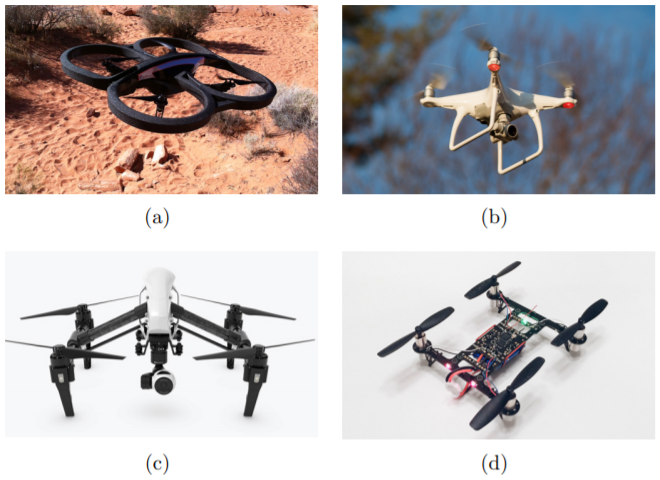
\includegraphics[scale=0.5]{images/droneExamples.PNG}
    \caption{Examples of multirotor UAVs \cite{zimmerman2016}}
    \label{fig:droneExamples}
\end{figure}

\section{An Overview of UAVs}
\begin{figure}[h]
    \centering
    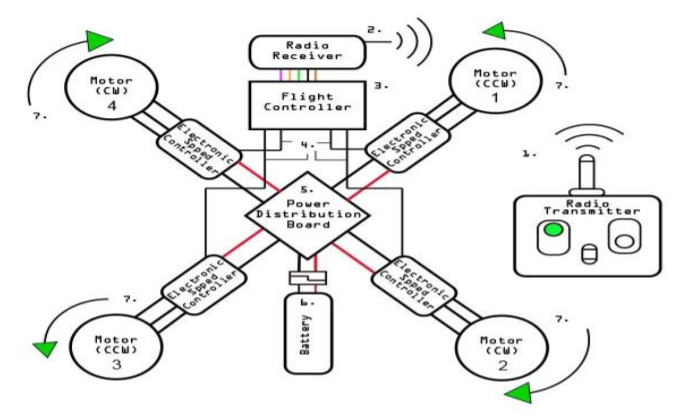
\includegraphics[scale=0.7]{images/fc_diag.PNG}
    \caption{Diagram of a quadcopter with radio transmitter\cite{fcDesign2019}}
    \label{fig:baseQuad}
\end{figure}
One might view the UAV as a black box where we input certain instructions and the UAV provides output in the form of
movement. Looking further into the system, we can see quite a bit of complexity with the internal subsystems that need
to interact in order for the UAV to achieve stable flight.
One of the most common types of multirotor UAVs is the quadcopter or quadrotor, so named because it uses four motors to
move around. The system diagram of a quadcopter may be seen in figure \ref{fig:baseQuad}. Some of the vital parts that all
multirotors have in common are:
\begin{enumerate}
    \item Motors
    \item Electronic speed controllers (ESCs)
    \item Battery
    \item Radio transceiver
    \item Flight controller
\end{enumerate}
The \textbf{motors} are the primary and often sole method of movement for the UAV. Coupled with propellers, they rotate at
very high velocities in order to generate lift. These motors are often brushless and generate high torque in exchange for
taking up a large amount of current \cite{fcDesign2019}. 
\newline
\newline
The \textbf{electronic speed controllers} are connected directly to the motors and allow you to control them through PWM
signals from the flight controller. There is typically one ESC for each motor \cite{zimmerman2016}. The ESC we will be 
using for the project is a 4-in-1 ESC board that can control four motors from one board. This was chosen as it was less
costly and more lightweight than using individual ESC modules. It is important to note that although the flight controller
can send data to the ESCs, the ESCs cannot provide direct feedback.
\newline
\newline
UAVs typically use lithium polymer \textbf{batteries}. Lithium polymer batteries are one of the densest commercially
available batteries in terms of energy \cite{LiPoly}. Because of this, they are lightweight and can provide the large 
amounts of current that is needed by the motors. In addition, the batteries also power the flight controller as well as
other onboard peripherals. In some instances, the flight controller may even read the voltage of the battery with respect to
its maximum operating voltage, thereby getting a sense of the remaining battery capacity.
\newline
\newline
The \textbf{radio transceiver} is the piece of hardware that allows the UAV to communicate with a base station. This allows
a pilot to send commands to the UAV and receive data such as telemetry or GPS coordinates \cite{zimmerman2016}.
\newline
\newline
The \textbf{flight controller} is, as its name suggests, the central device that controls how the UAV moves and reacts to certain
stimuli. The flight controller contains multiple sensors including (but not limited to) a gyroscope, accelerometer, and
barometer. These sensors allow the flight controller to get a sense of its orientation in 3D space \cite{zimmerman2016}. The
flight controller sends instructions to the ESCs in order to vary the throttle of each motor.

\section{A Deeper Look Into Flight Controllers}
Because of the growing interest in UAVs, various flight
controllers have been developed such as the microcontroller-based Multiwii \cite{MultiwiiFC} and PixHawk \cite{RPiMavlink2019}.
Microcontroller based flight controllers are ideal because they are lightweight, low-cost, and are generally versatile enough
to accomodate the peripherals that a flight controller needs in order to function properly. On top of this, these flight controllers
are often open-source and relatively simple to prototype with. However, due to the limited processing power available to 
microcontroller based flight controllers, higher level functions such as automated navigation or mapping are often impossible 
without the help of an onboard computer (often a Raspberry Pi) communicating directly with the flight controller 
\cite{RPiMavlink2019,Redtail2017,Dowling2018,Navio2,AirPy}.
\begin{figure}[h]
    \centering
    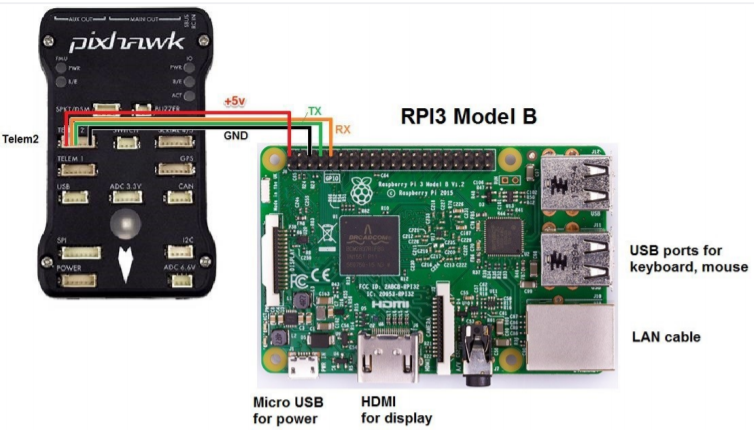
\includegraphics[scale=0.5]{images/phawkToPi.PNG}
    \caption{Connecting a Pixhawk flight controller to a Raspberry Pi \cite{RPiMavlink2019}}
    \label{fig:phawkToPi}
\end{figure}
Curiously, while there are numerous flight controllers based off of microcontrollers, there are no publicly available flight 
controllers that directly utilize an onboard computer to interface with the electronic speed controllers, thereby skipping
the microcontroller entirely. Doing so would not only lower the cost of producing the flight controller, but it would also
reduce the flight controller's size and weight while still allowing access to higher level UAV functions. A solution to this
would be to develop a flight controller board built around the Raspberry Pi 4, which is the latest and currently most powerful
version of the Raspberry Pi line of computers. Doing so involves designing and fabricating the flight controller board (with
the necessary peripherals) as well as modeling and programming the control system. In order to make the UAV easy to mass produce 
and more affordable, production cost was prioritized while designing the flight controller. 


\chapter{Review of Related Work}
As mentioned previously, a vast majority of commercially available flight controllers are based on microcontrollers. In order to
adapt this technology to single board computers such as the Raspberry Pi, it would serve well to examine microcontroller based
implementations. We will first look into the system architecture and design on a hardware level before moving on to how to model
the control system and program it into the hardware.
\section{Hardware Design}
Looking into open-source microcontroller-based flight controllers, two of the most prominent ones are the MultiWii \cite{MultiwiiFC}
and the PixHawk family of flight controllers \cite{RPiMavlink2019}. The MultiWii is the more dated of the two systems and the PixHawk
may also trace its origins to it. The MultiWii was
developed to use the Arduino line of microcontrollers as a base though it can also run on other select microcontrollers. It also
supports a variety of inertial measurement units (IMUs), which are sensor modules that carry an accelerometer and gyroscope and,
for some modules, even a magnetometer or barometer \cite{zimmerman2016}. Figure \ref{fig:multiwiiCktDiagram} illustrates the circuit
diagram of a basic MultiWii quadrotor UAV. In this digram, we can see that the flight controller is connected to four electronic speed
controllers (ESCs) which then control the motors directly. The flight controller takes inputs from a receiver, detailing the levels
of throttle, roll, pitch, and yaw as well as a few auxiliary channels which may be used for other functions such as LEDs or arming
the motors. The flight controller also makes use of an IMU in order to get a sense of its orientation. Along with the signals from
the receiver, it feeds this data into a PID loop (which will be discussed further on in this document) in order to maintain stable flight
\cite{zimmerman2016}. Thus, we can infer the most important parts of a flight controller; the flight controller board and the IMU.
\begin{figure}[h]
    \centering
    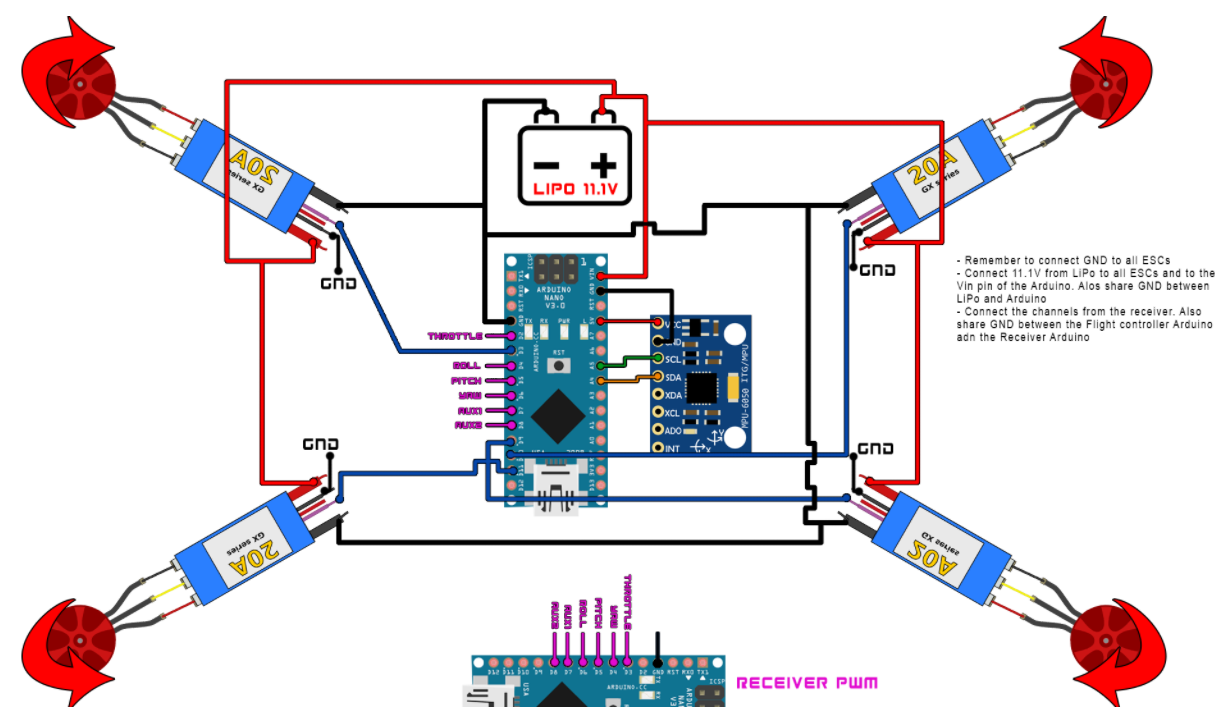
\includegraphics[scale=0.5]{images/multiwii diagram.PNG}
    \caption{Circuit diagram of basic MultiWii multirotor UAV \cite{MultiwiiFC}}
    \label{fig:multiwiiCktDiagram}
\end{figure}
\newline
\newline
Taking a step further, Sigalos et al. verify our inference in their paper entitled "Design of a Flight Controller and Peripherals 
for a Quadcopter" \cite{fcDesign2019}. As seen in figure \ref{fig:baseQuad}, the diagram is very similar to that of the base MultiWii. 
The biggest difference would be the addition of a power distribution board. The power distribution board is essentially just a circuit board
where the ESCs may be connected together. This would allow us to use less wires, thereby making the physical system tidier and thus 
easier to manage. It is also important to note that the battery voltage must be stepped up or down depending on the working voltage of
the chosen controller. In the case of the MultiWii, the battery used is a 11.1V Lithium Polymer battery. The author states that a voltage
converter was no longer needed as 11.1V is within the acceptable input voltage range of the Arduino Nano which the implemented MultiWii
uses. The Arduino Nano also already comes with an internal voltage regulator capable of stepping down the 11.1V to a more manageable
voltage. This, however, is not the case when working with the Raspberry Pi, where the input voltage must not exceed 5.1V. Thus, a
voltage regulator must be integrated into the flight controller.

Zimmerman illustrates this more clearly in their thesis "Flight Control and Hardware Design of Multi-Rotor Systems". In figure 
\ref{fig:detailed_quad_block_diagram}, the microcontroller used in the flight controller has a working voltage of 3.3V, which is a far cry
from the 11.1V input voltage. In order to compensate for this, they use a low dropout regulator to step the input voltage down to 3.3V. It
is also important to note that the microcontroller communicates both with the IMU and radio receiver via SPI. The designed flight controller
also has interfaces for PPM and UART which, as seen from the electrical architecture, were used for sonar and lidar respectively. Lidar and
sonar, however, are not vital to the UAV's operation and are treated as peripherals. It is also to be noted that this implementation does
not have an available I2C interface, something that the Raspberry Pi supports natively. The presence of an I2C interface would allow the
UAV to access more sensors or external modules should they become necessary for the UAV's application.
\begin{figure}[h]
    \centering
    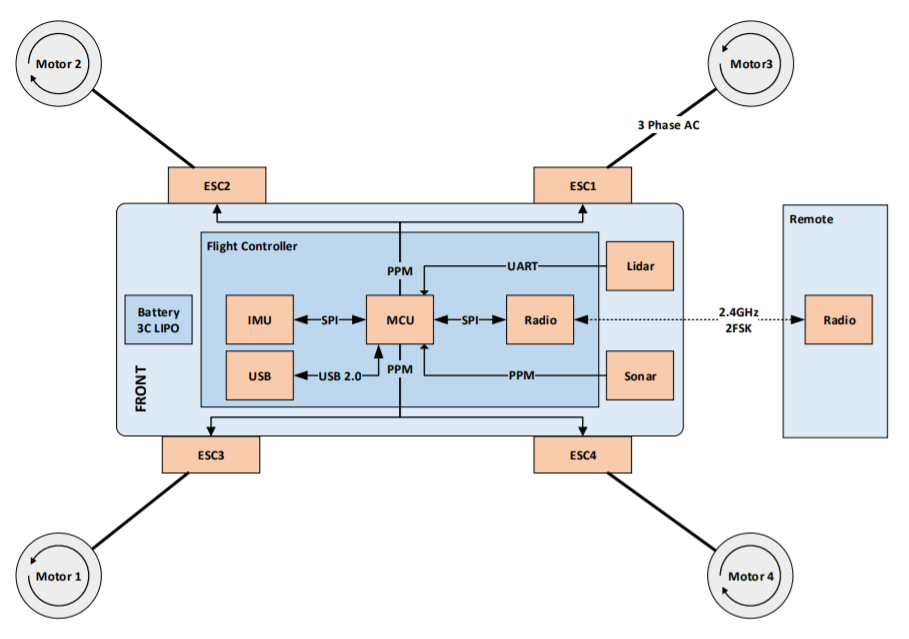
\includegraphics[scale=0.45]{images/zimmerman_high_level.PNG}
    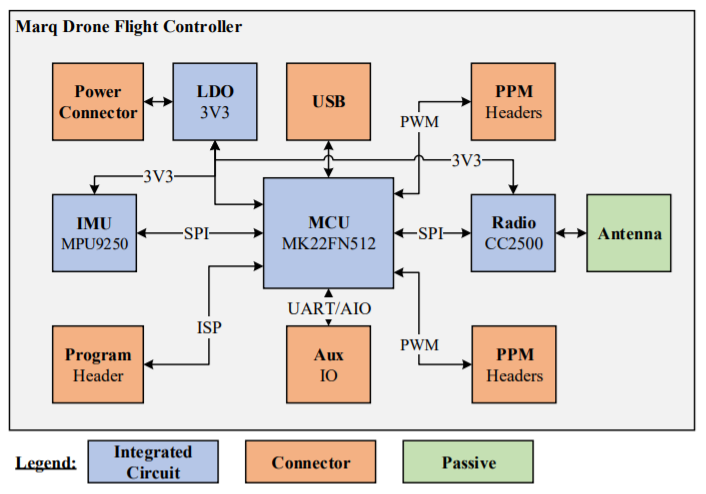
\includegraphics[scale=0.45]{images/fc_block_diagram_detailed.PNG}
    \caption{Electrical architecture diagram (left) and corresponding flight controller block diagram (right)\cite{zimmerman2016}}
    \label{fig:detailed_quad_block_diagram}
\end{figure}
\newline
\newline
Perhaps the device that best resembles what this project is trying to accomplish is the Navio2 \cite{Navio2}. Developed by a company called
Emlid, the Navio2 was designed to plug directly onto the Raspberry Pi, allowing it to function as a flight controller in and of itself. It
has two built-in IMUs as well as a barometer and a GPS module. It also supports UART as well as I2C. It does not have a built in power
module and thus any input voltage larger than 5.1V must still be stepped down accordingly. Because the Navio2 was developed for an older
version of the Raspberry Pi (namely the Raspberry Pi 2), it still needs to account for the lack of processing power. It does this by
making use of an integrated microcontroller to handle the low-level functions such as processing the PPM input from the radio receiver.
Ultimately, the Navio2 was designed more to be a solution for easy-to-use autopilot rather than a standalone flight controller. 
\begin{figure}[h]
    \centering
    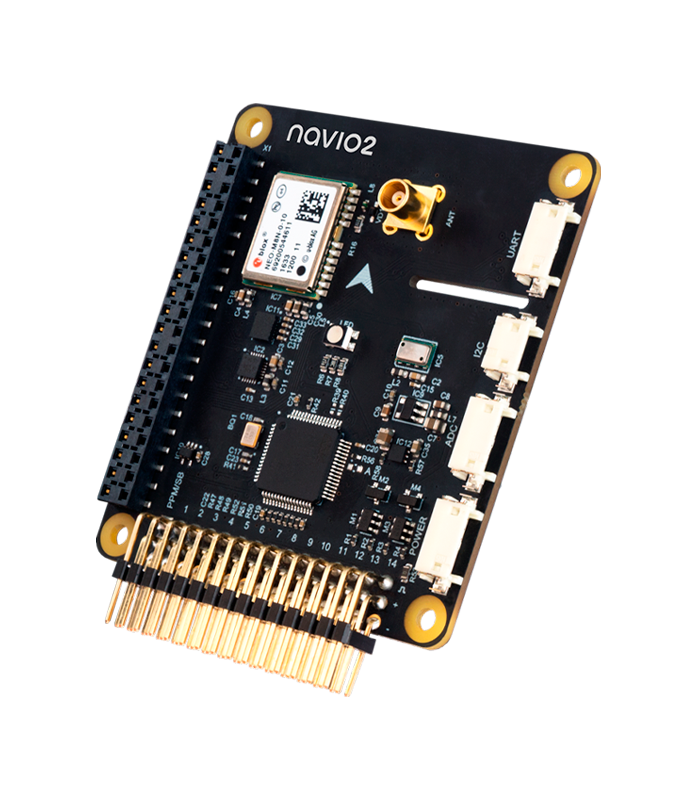
\includegraphics[scale=0.3]{images/Navio2Elements_main.png}
    \caption{Navio2 Raspberry Pi hat \cite{Navio2}}
    \label{fig:navio2}
\end{figure}

\section{Control System Design and Programming}
In typical multirotor UAV designs, the motor positions are static with respect to each other. This means that it is not possible to change
the direction of an individual motor in order to influence flight. Instead, the UAV changes the angular velocity, $\omega$, of each motor according to
the direction the pilot would like to go \cite{fcDesign2019}. Figure \ref{fig:motor_signals} gives us an idea of how adjusting the angular
velocities of the individual motors affects the direction the UAV will fly in. First, it is important to note that not all of the motors
(and by extension- the propellers) are rotating in the same direction. Using figure \ref{fig:motor_signals} as a reference, you would
typically have motors 1 and 3 rotating counter clockwise while motors 2 and 4 rotate clockwise. This is because the rotation of the motors
generates torque. If they were all rotating in the same direction, the entire UAV would continue to rotate. Thus, having the motors rotate
in opposing directions would negate that torque. 
\begin{figure}[h]
    \centering
    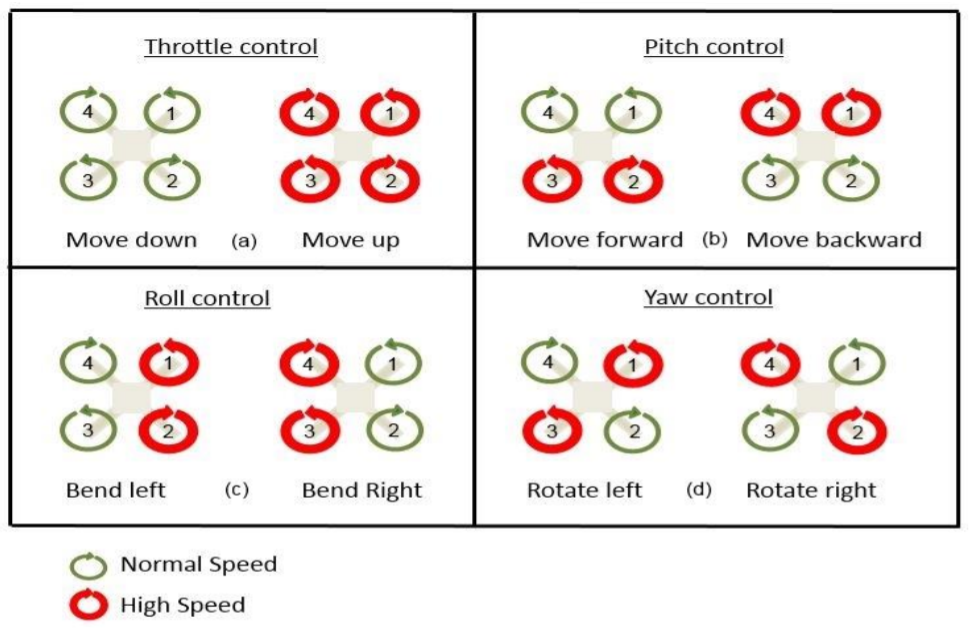
\includegraphics[scale=0.5]{images/motor_signals.PNG}
    \caption{Controlling the UAV \cite{fcDesign2019}}
    \label{fig:motor_signals}
\end{figure}
\newline
In order to be able to model the system and define the control objectives, it is important to get a sense of the parameters that determine
how the UAV moves. For that, we have throttle, pitch, roll, and yaw. These are all illustrated by figure \ref{fig:motor_signals} a, b,
c, and d respectively. Throttle dictates the angular velocity of all of the motors. It affects flight velocity as well as the altitude of the
UAV. Pitch is what allows the UAV to move forward or backward. In order to move forward, the flight controller would instruct motors 2 and 3
to accelerate while keeping motors 1 and 4 at a constant angular velocity. The opposite is true for flying backwards. Meanwhile, roll controls
lateral movement. In order to fly to the left, the flight controller would instruct motors 1 and 2 to accelerate while keeping motors 4 and 3
at constant velocity. The opposite is once again true for flying to the right. Perhaps most interesting would be how yaw controls the direction
that the UAV is facing. It was previously discussed that the opposing motor orientations allow the UAV to negate the torque and obtain stable
flight. Yaw takes advantage of this by accelerating either the clockwise rotating motors or the counter-clockwise rotating motors in order to
rotate right or left respectively.
\newline
\newline
With the parameters defined, Zimmerman presents a frame of reference for the UAV \cite{zimmerman2016}. This may be seen in figure \ref{fig:ref_frame}
\begin{figure}[h]
    \centering
    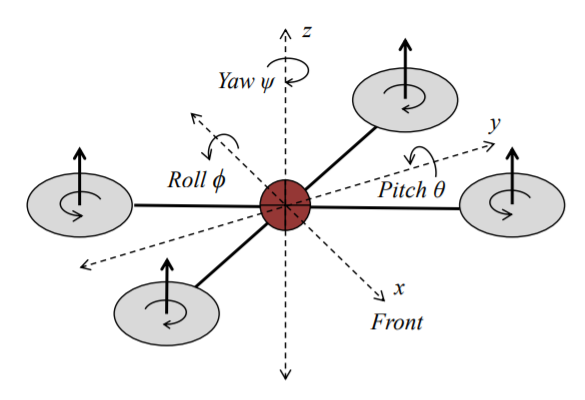
\includegraphics[scale=0.5]{images/quad_ref_frame.PNG}
    \caption{UAV reference frame \cite{zimmerman2016}}
    \label{fig:ref_frame}
\end{figure}
They define pitch to be $\theta$, roll to be $\phi$, yaw to be $\psi$, and throttle to be $T$. These are the current values of the parameters.
They then define $\theta_c$ to be the user commanded pitch, $\phi_c$ to be the user commanded roll, $\psi_c$ to be the user commanded yaw, and
$T_c$ to be the user commanded T. Lastly, they define $ \dot{\theta}, \dot{\phi}, \dot{\psi}$ to be the rotational velocities. According to
Zimmerman, the first set of control goals may be summarized by equation \ref{eq:ctrl_goals_1}.
\begin{align}
    \dot{\theta}&=0                      &  \dot{\phi} &=0                 &  \dot{\psi}&=0\\
    \label{eq:ctrl_goals_1} 
    \theta &\rightarrow \theta_c         & 
     \phi &\rightarrow \phi_c       &  \psi &\rightarrow \psi_c &  T &\rightarrow T_c
\end{align}
In essence, the goal of the flight controller is to drive the parameters to the user specified values. Using these four parameters, the user
is able to maneuver the UAV anywhere in 3D space. In order to achieve the control goals, a PID controller system is implemented. A PID controller is a
control system that updates based on the desired output and the measured output \cite{zimmerman2016}. "PID" stands for proportional, integral,
and derivative. This is because the system has three coefficients (P, I, and D) that characterize how the system reacts to proportional, integral, 
and derivative errors. In their thesis, Zimmerman designed a base PID system with the UAV acting as the plant as seen in figure \ref{fig:basePID}.
\begin{figure}[h]
    \centering
    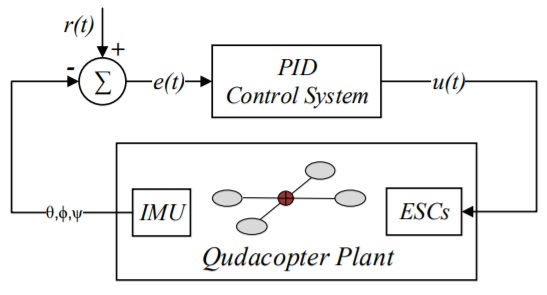
\includegraphics[scale=0.5]{images/basePID.PNG}
    \caption{Diagram of UAV plant and control system \cite{zimmerman2016}}
    \label{fig:basePID}
\end{figure}
Here, r(t) is denoted as the desired setpoint or the user commanded value. e(t) is the error or difference between the output of the UAV plant and
r(t), and u(t) is the input to the plant after the error goes through the PID control system. As we can see, this system also takes into account
the IMU and ESCs for feedback. The ESCs are updated according to u(t) and the corresponding movement is measure by the IMU in order to process it
once again. However, as Zimmerman states, this system is only valid for one parameter. Therefore, there must be one system for each of pitch, roll, 
and yaw. The system is linearized at a current point in time and therefore superposition is upheld. They expand on the control system shown in 
figure \ref{fig:basePID} by incorporating each parameter as well as illustrating how the user commanded throttle $T_c$ fits in the picture. 
\begin{figure}[h]
    \centering
    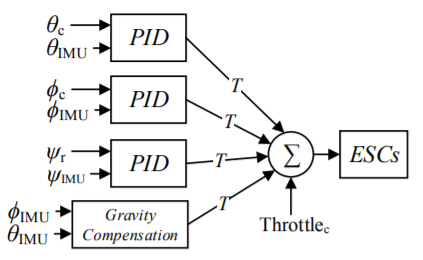
\includegraphics[scale=0.65]{images/controlSysExpanded.PNG}
    \caption{Expanded view of UAV control system \cite{zimmerman2016}}
    \label{fig:expandedPID}
\end{figure}
As we can see from figure \ref{fig:expandedPID}, each PID block takes in the user commanded value of the parameter as well as the parameter's
feedback from the IMU. It then takes in the summation of all of the PID outputs with the user commanded throttle and sends the information to the
ESCs. Zimmerman then goes on to explain how a code for the system may be written for the microcontroller they used for the thesis. While the code
isnt directly compatible with the Raspberry Pi due to differing system architectures, the code was used as a basis to adapt a version capable
of running on the Raspberry Pi.
\newline
\newline
Now that a control system has been established, there is still the issue of which PID coefficients to use. In order to determine the coefficients,
UAVs often undergo tuning. This is especially important for pilots involved in the sport of drone racing as the UAV's PID coefficients heavily
impact its flight characteristics \cite{Dowling2018}. One method of tuning a UAV is by conducting test flights where the pilot executes sharp
maneuvers, subjecting the UAV's IMU to drastic changes and seeing how the UAV reacts or how quickly it stabilizes \cite{Tuning2017}. Once the tests
are conducted, the pilot would then promptly land and plug the flight controller into a computer to update the PID coefficients in a trial-and-error
manner. One benefit of using a single-board computer rather than a microcontroller for a flight controller is that there would no longer be a need
to plug the flight controller into a separate computer just to update the coefficients. This may now be done mid-flight


\chapter{Problem Statement and Objectives}
With the rise of research involving multirotor unmanned aerial vehicles comes the development of more advanced flight controllers to aid in the
fabrication of these UAVs. Most (if not all) open source flight controllers are based on microcontrollers while there are no flight controllers
built around single-board computers. Developing a flight controller built around a single-board computer would provide the UAV with access to 
higher level functions such as automated navigation while being lighter and less expensive than microcontroller based flight controllers that
attempt to implement the same higher level functions.
\newline
\newline
This project aims to develop a general purpose flight controller built around the Raspberry Pi and without integrating an auxiliary microcontroller.
To do this, the following objectives must be achieved: 
\begin{enumerate}
    \item The flight controller should be capable of running on a Raspberry Pi 4 without using an auxiliary microcontroller.
    \item The flight controller should be able to sustain stable flight, maintaining a mean error for each parameter (pitch, roll, yaw) of at most 0.001\textdegree
        and a standard deviation of at most 0.4816\textdegree.
    \item The flight controller should be able to respond to commands given by the base station and send back telemetry data.
\end{enumerate}

\chapter{Methodology}
\section{System Overview}
\begin{figure}[h]
    \centering
    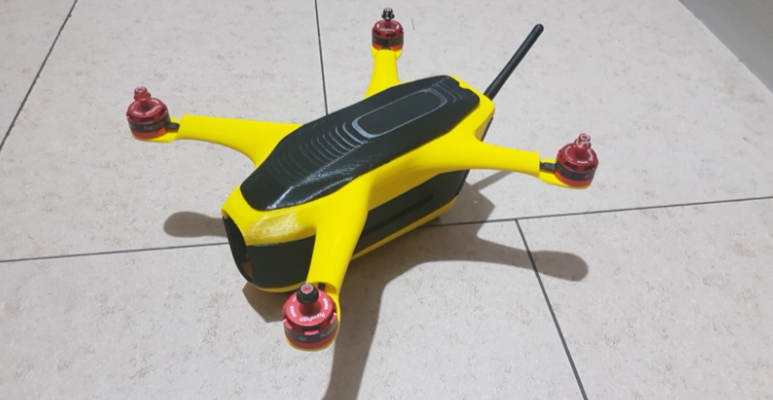
\includegraphics[scale=0.5]{images/diosa_full.PNG}
    \caption{Project Diosa prototype chassis with electronics installed}
    \label{fig:diosa_full}
\end{figure}
A system was designed and fabricated reflecting the diagram seen in figure \ref{fig:final_FC_diagram_na}. As we can see,
the Raspberry Pi draws inertial data directly from the IMU and gathers geographical coordinates from the GPS whenever there is a GPS
signal available. GPS is typically only available outdoors. The Raspberry Pi is also directly connected to the ESCs, giving
the Raspberry Pi full authority over them. This is in contrast with microcontroller based flight controllers, where an onboard computer
may only send certain signals. A half duplex radio connection was established between the flight controller and a base station. 
This allows the flight controller to take commands from the base station whilst simultaneously sending back telemetry data for 
in-flight debugging.
\begin{figure}[h]
    \centering
    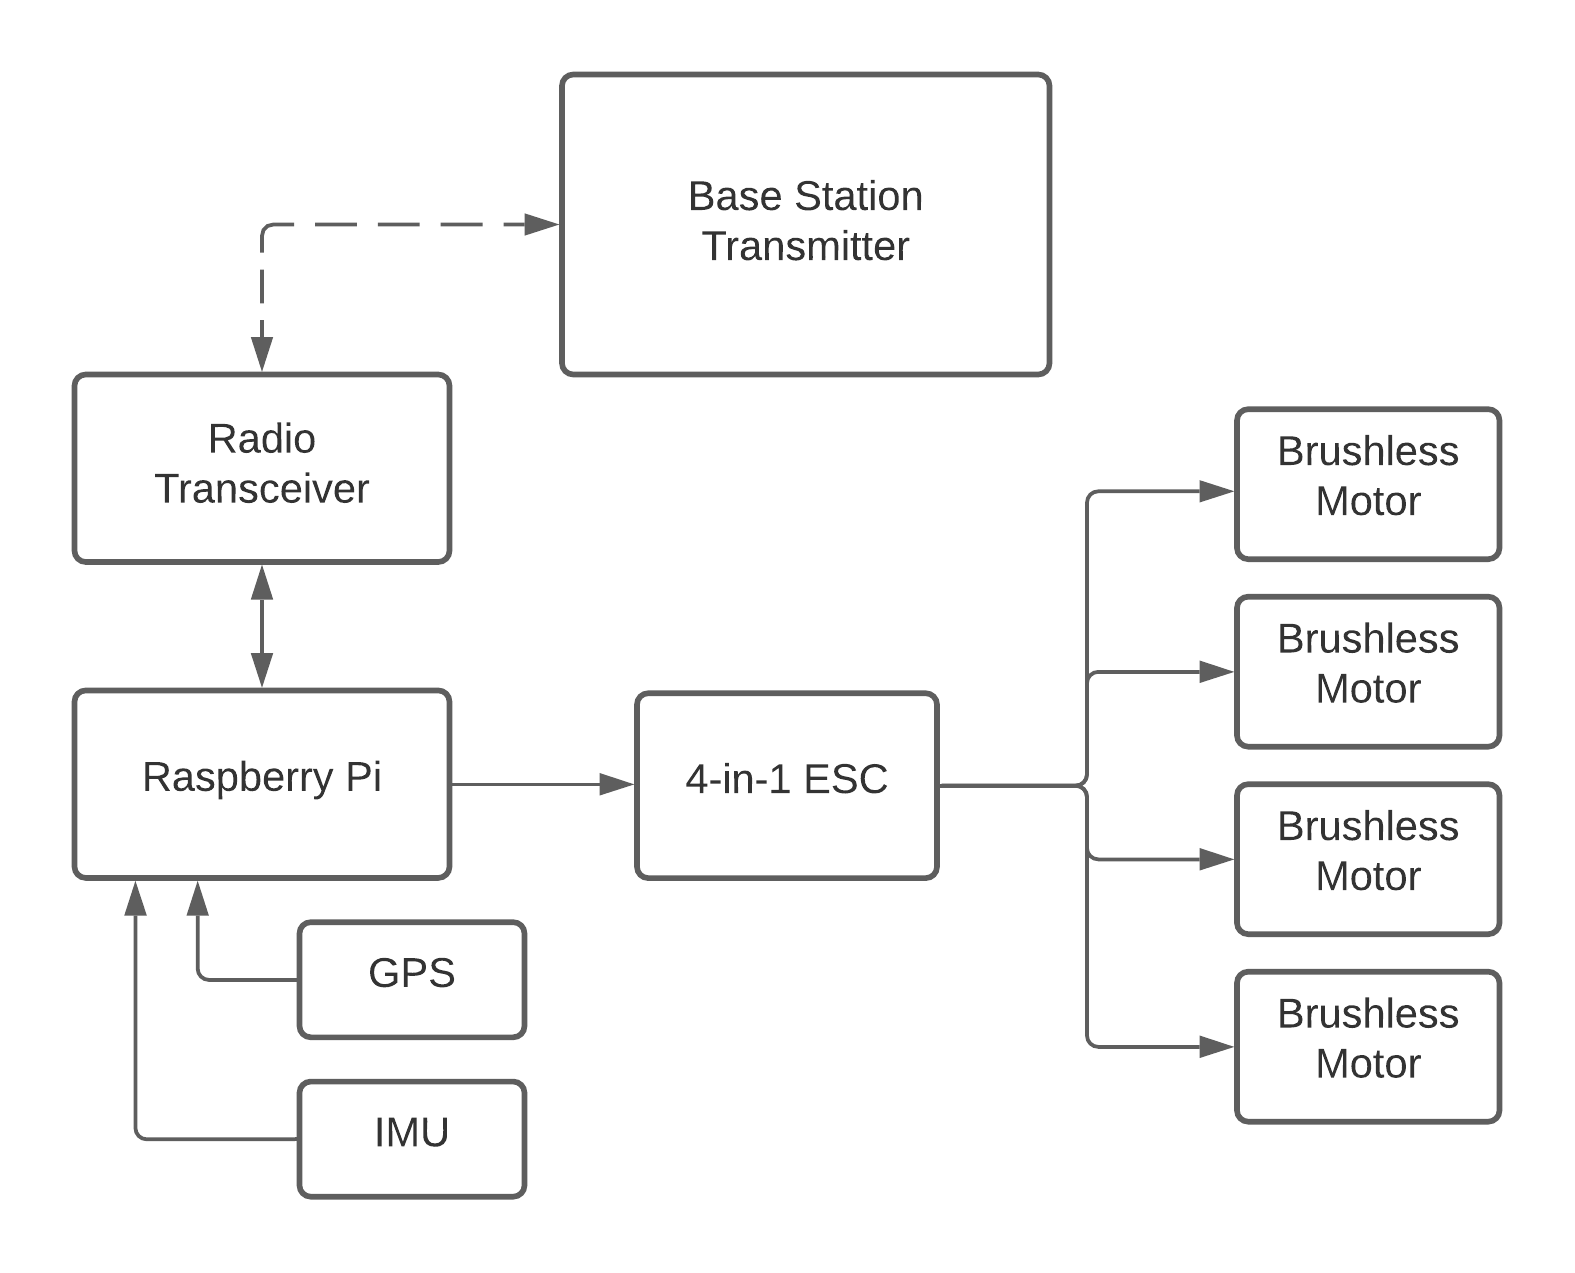
\includegraphics[scale=0.5]{images/FC diagram_finalna.png}
    \caption{Flight controller diagram with ESC module and motors}
    \label{fig:final_FC_diagram_na}
\end{figure}
With the system established, the designed control system was then adapted into code to be run on the Raspberry Pi. 
Integration of the PID control system into the flight control code was done with aid from Zimmerman's 
derivation and code of his own system \cite{zimmerman2016}. Once the PID control system was established, the other basic 
functions were developed. The ADC was set up such that it can measure the battery voltage. This allows the UAV to
send the battery level back to the base station. This function is important as it is vital that the pilot knows how much battery
(and by extension, flight time) the UAV still has. The GPS module was also set up in such a way that the UAV is able to
send its current coordinates back to the base station in the event that a GPS signal is detected. This function is vital for
tracking the UAV in the event of a crash.

\subsection{ROS Implementation}
The Raspberry Pi is running the latest version of Raspbian, which, at the time of this writing, is Raspbian Buster. The control system itself is coded in Python 3.7 and
uses ROS Noetic Ninjemys \cite{ROSNoetic} as the base framework. ROS was chosen for its modularity and language agnosticism, allowing us
to code in either Python or C++ and even allowing the two types of programs to work seamlessly with each other. One of the core functions
of ROS is its publisher/subscriber system, where multiple programs may send each other packets of data by publishing and subscribing to
certain nodes that ROS calls "topics". 
\begin{figure}[h]
    \centering
    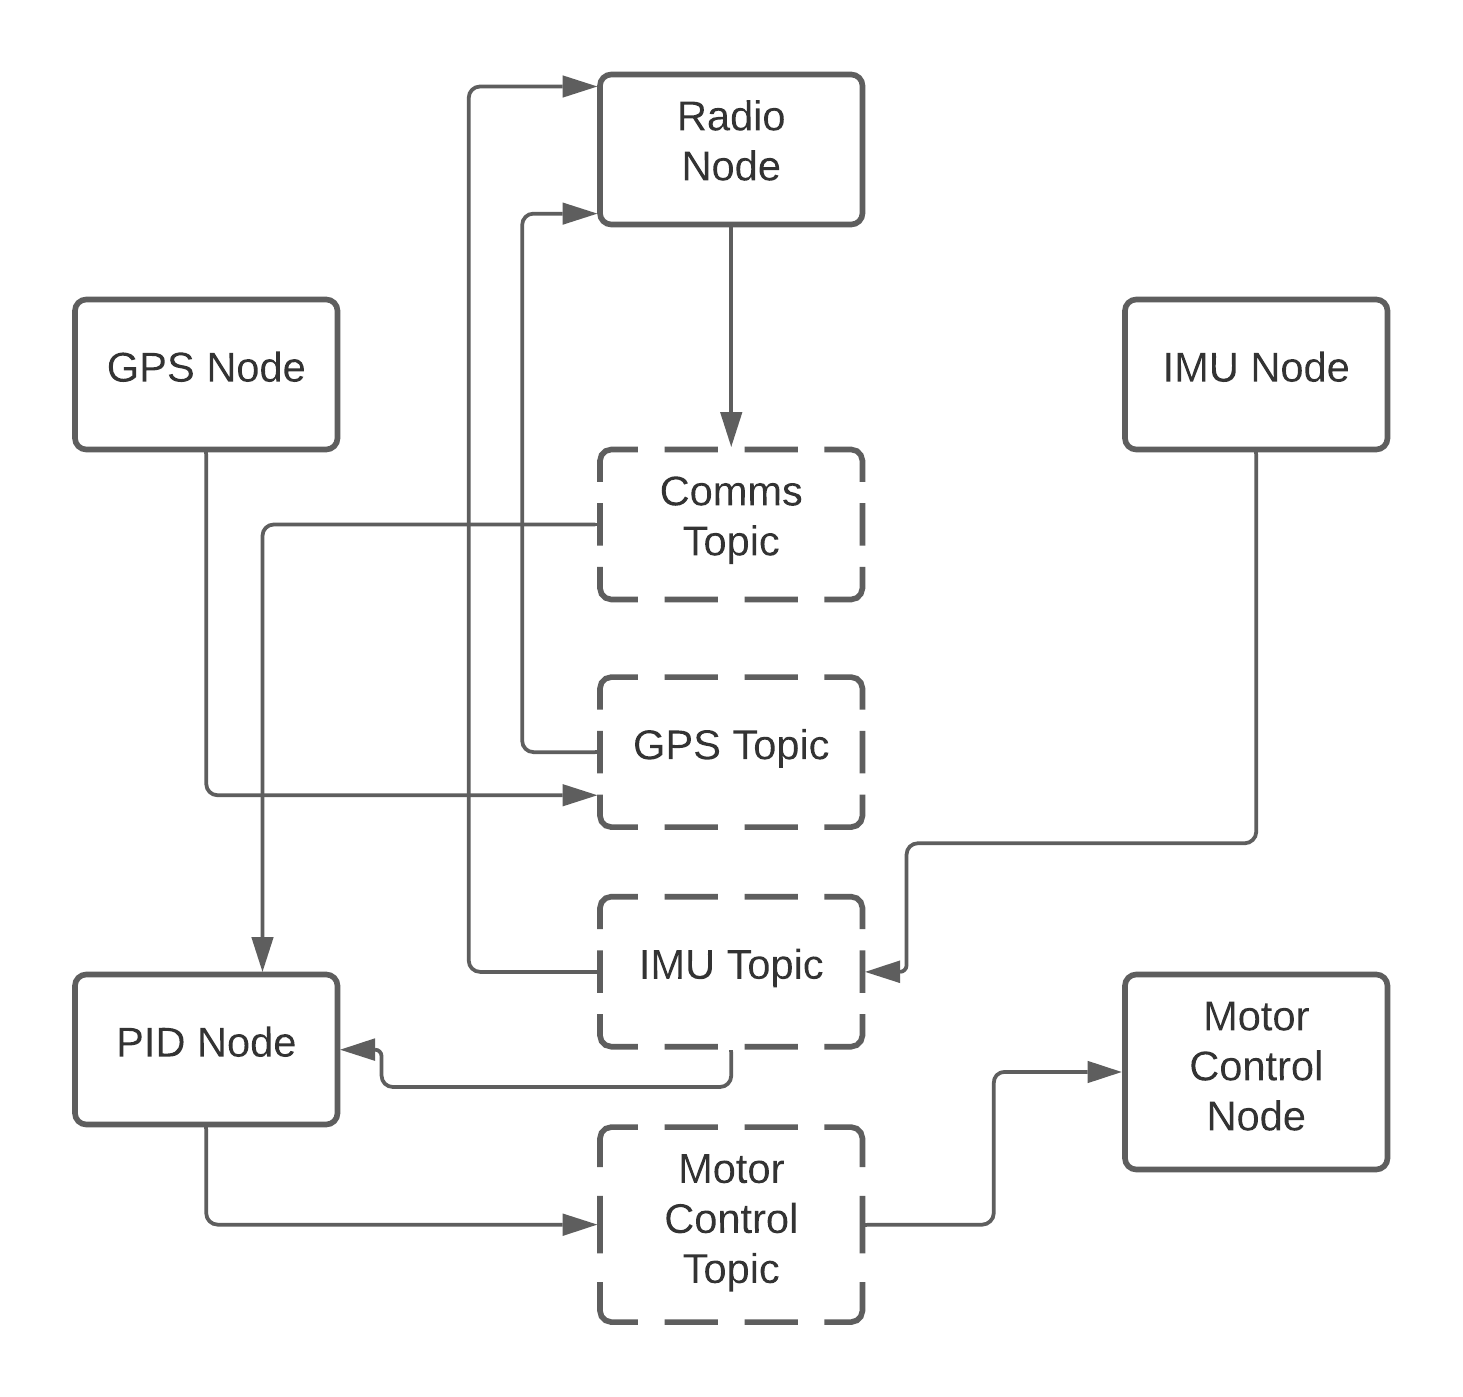
\includegraphics[scale=0.6]{images/rostopics.png}
    \caption{Diagram of ROS nodes and topics}
    \label{fig:ros_topics}
\end{figure}
Figure \ref{fig:ros_topics} shows a diagram of how the ROS nodes interact with the different topics in order to pass around data.
There are five nodes communicating with four topics. The first node is the radio node, which handles communications with the base station. It
takes incoming transmissions from the flight controller's transceiver module and broadcasts the data onto the comms topic. The comms topic
typically pertains to data regarding the desired throttle, roll, pitch, yaw, and auxiliary switches. This data is primarily used in conjunction
with the IMU data to calculate the necessary motor speeds in the PID node. The IMU node simply takes measured data from the flight controller's
IMU and broadcasts it to the IMU topic. Data from the IMU topic also flows into the radio node so that it can send the data back to the base
station, giving the pilot real-time data on the UAV's actual pitch, roll, and yaw values. Once the PID node has data from the IMU and the
transceiver, it then calculates the necessary motor speeds and broadcasts them to the motor control topic, which the motor control node is 
subscribed to. The motor control node updates the ESCs accordingly. Lastly, we have the GPS node and GPS topic. The GPS node pertains directly
to the flight controller's GPS module and, if a signal is available, broadcasts the UAV's coordinates to the GPS topic. Data from the GPS topic
is sent to the radio node, allowing the flight controller to send the UAV's coordinates back to the base station.

\subsection{Base Station and Flight Controller Communication}
The flight controller and the base station share a half-duplex connection using a pair of nRF24L01 2.4GHz RF transceiver modules\cite{EDWNrf24}. The LoRa Ra-02
was previously considered however, at 433MHz, the frequency was deemed too low. While a higher frequency was reached with the nRF24L01, the
effective range decreased from 10km to 1km. 
\begin{figure}[h]
    \centering
    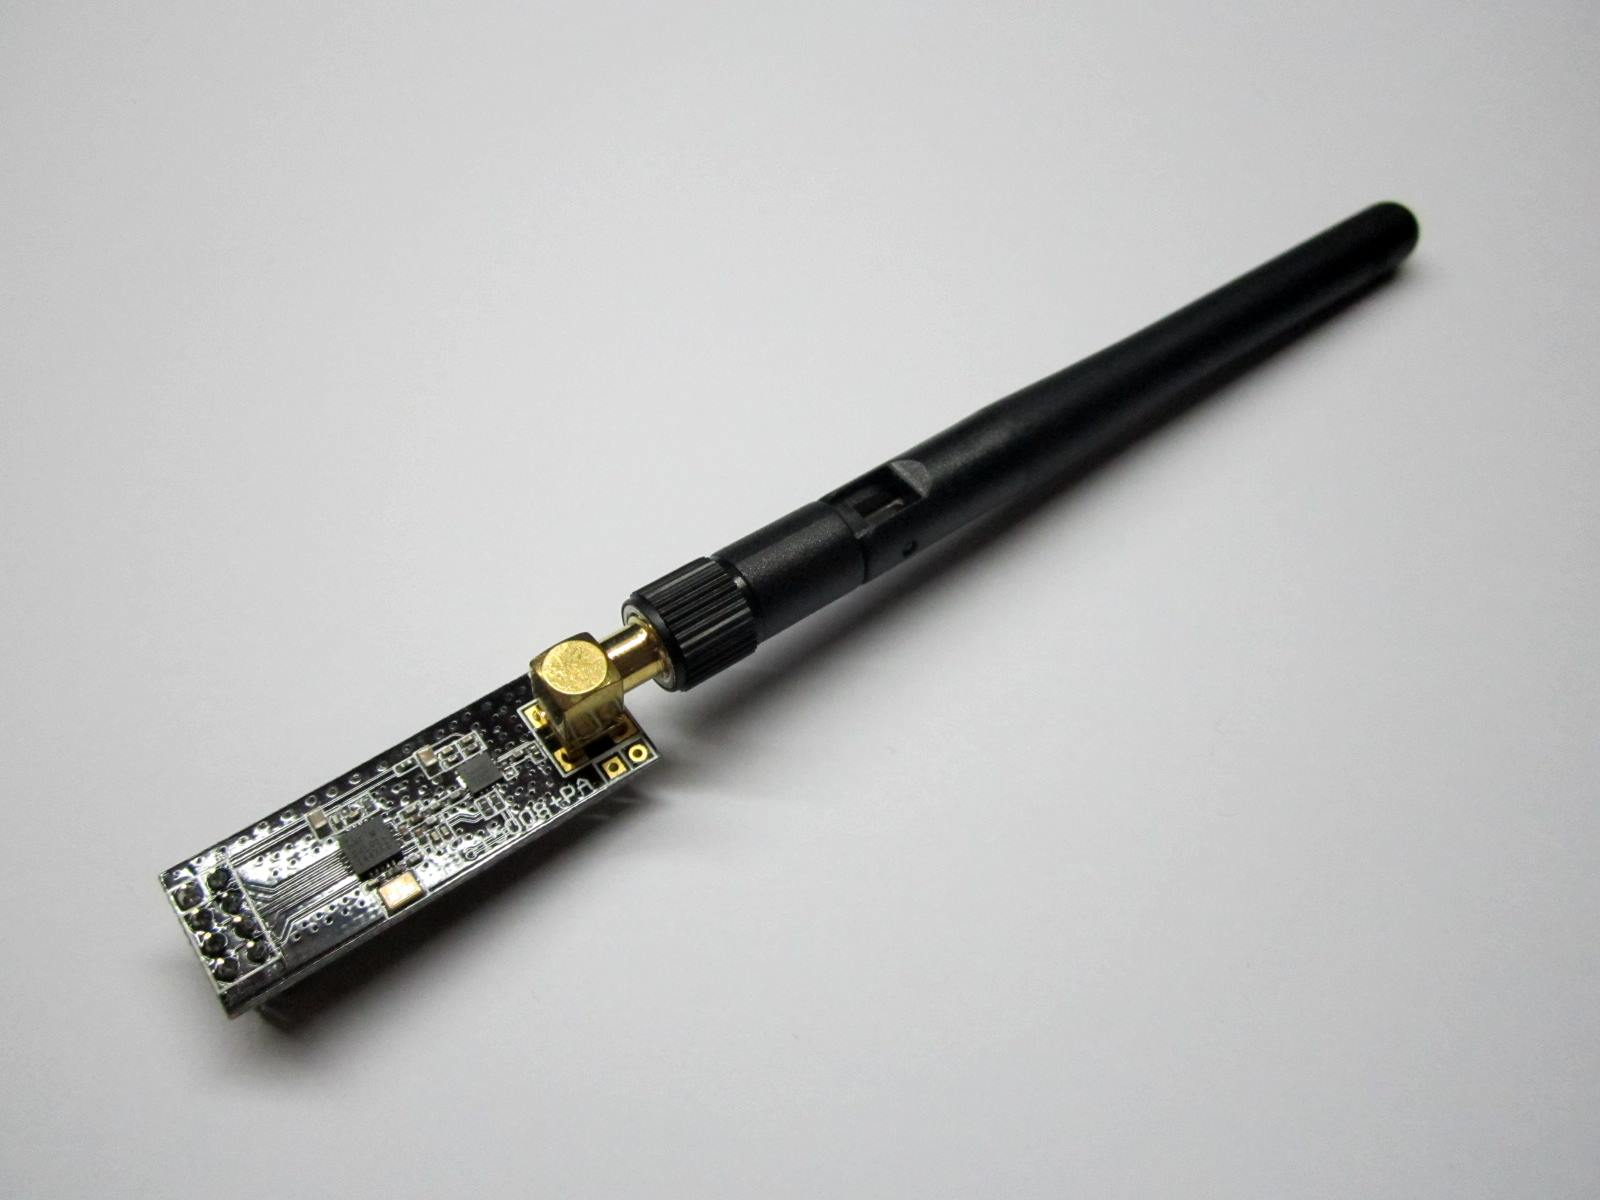
\includegraphics[scale=0.3]{images/nrf24.jpg}
    \caption{nRF24L01 transceiver module with antenna\cite{EDWNrf24}}
    \label{fig:nrf24}
\end{figure}
\begin{figure}[h]
    \centering
    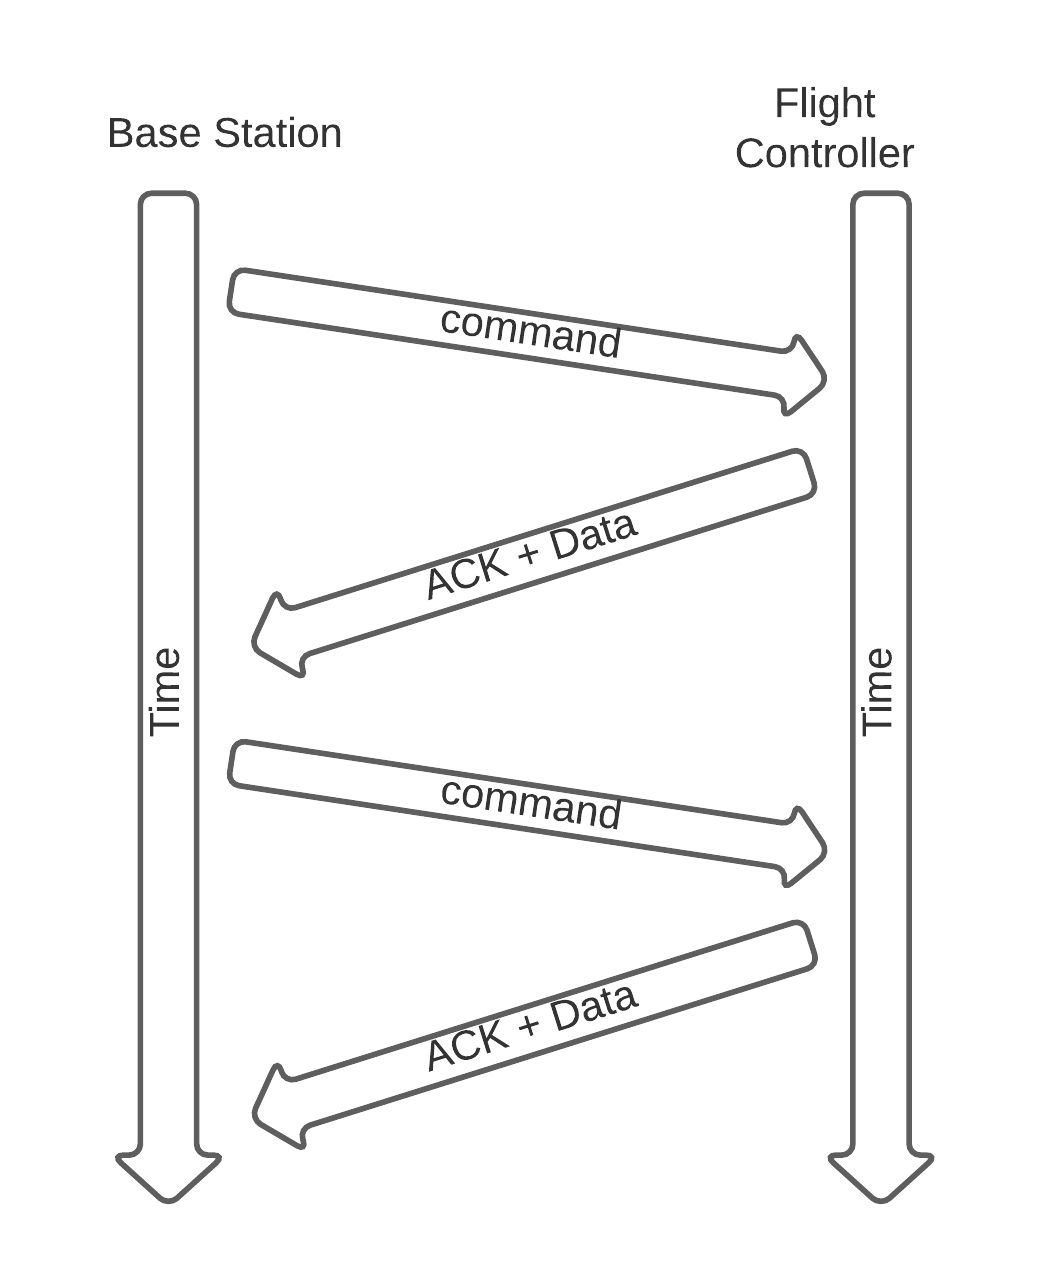
\includegraphics[scale=0.6]{images/commsSetup.png}
    \caption{Diagram of communication between base station and flight controller over time}
    \label{fig:commsSetup}
\end{figure}
\newline
\newline
Figure \ref{fig:commsSetup} illustrates how the flight controller and base station communicate over time. From a client / server standpoint, the
base station acts as a client while the flight controller acts as a server. The base station repeatedly sends commands to the flight controller.
Once the flight controller receives a command, it then sends back an acknowledgement packet that also contains relevant data. The packet that the
base station sends to the flight controller contains the desired throttle, roll, pitch, yaw, and the state of four auxiliary switches that may be
programmed for various purposes. Meanwhile, the flight controller sends back the actual or measured pitch, roll, and yaw from the IMU as well as
the GPS coordinates.

\subsection{GPS Integration}
GPS integration was rather straightforward. The GPS module used was the UBLOX NEO-6M GPS Module \cite{EDWGPS}. Perhaps the biggest hurdle for the
GPS integration was that it would not be available while indoors. Because there was still a desire to track the location of the UAV while indoors,
we could at least remember its last known position. The solution to this was to simply store the latest obtained coordinates and update them only
when a desirable GPS signal was found.
\begin{figure}[h]
    \centering
    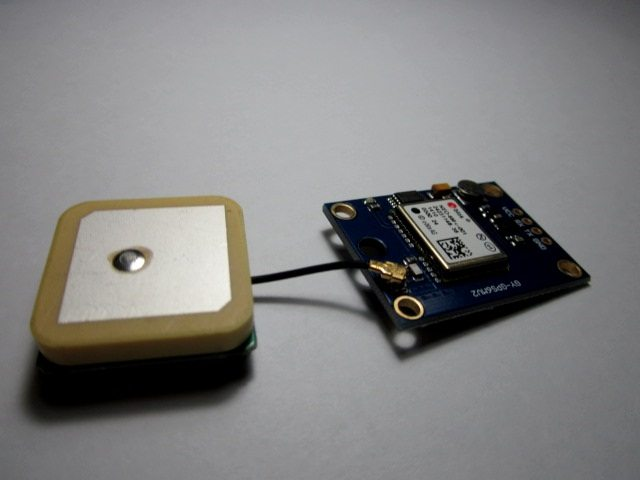
\includegraphics[scale=0.3]{images/gps_module.jpg}
    \caption{UBLOX NEO-6M GPS Module\cite{EDWGPS}}
    \label{fig:gps_module}
\end{figure}

\subsection{IMU Integration}
The inertial measurement unit used for the project was the GY-88 IMU \cite{EDWIMU} which includes a gyroscope, magnetometer, accelerometer, and
altimeter. As discussed previously, the IMU allows us to measure the UAV's angles of rotation about the X, Y, and Z axes. The purpose of using
multiple sensors is that it allows us to achieve a greater degree of accuracy. The question now would be how to integrate the data from the
multiple sensors into our desired output, which is in degrees of rotation. Fortunately, Zimmerman \cite{zimmerman2016} provides a rather
straightforward method of doing so. 
\newline
\newline
First, the results from the accelerometer were obtained using equations \ref{eq:pitch_eq} and \ref{eq:roll_eq}.
These two equations will respectively give the measured pitch and roll from the accelerometer. \(A_{x}\), \(A_{y}\), and \(A_{z}\) are the
acceleration readings along those respective axes which are read in Gs.

\begin{figure}[h]
    \centering
    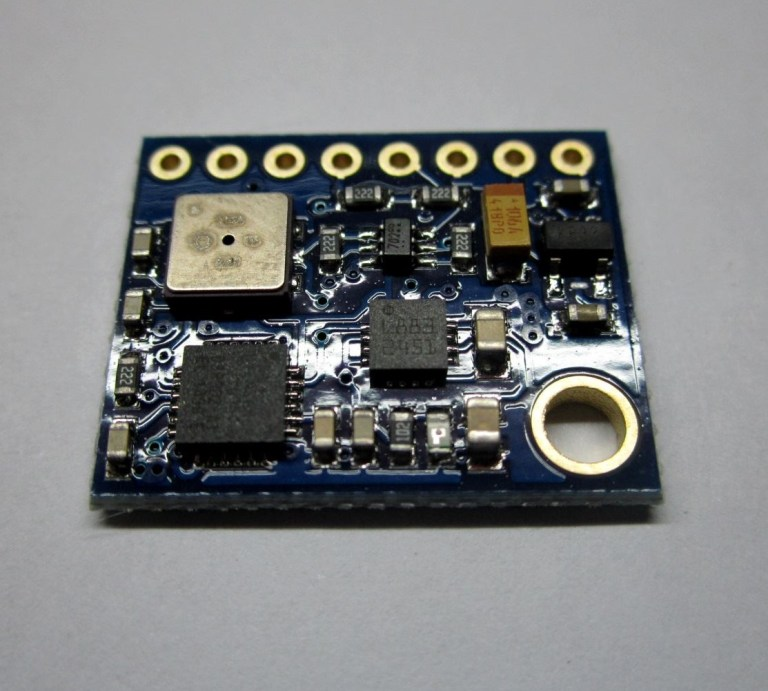
\includegraphics[scale=0.25]{images/imu_module.jpg}
    \caption{MPU6050+HMC5883L+BMP180 Gyro/Magnetometer/Accelerometer/Altimeter Sensor Module\cite{EDWIMU}}
    \label{fig:imu_module}
\end{figure}
\begin{equation}
    Pitch_{accel} = \arctan(\frac{A_{y}}{\sqrt{A_{x} + A_{z}}}) * \frac{180}{\pi}
    \label{eq:pitch_eq}
\end{equation}
\begin{equation}
    Roll_{accel} = \arctan(\frac{A_{x}}{\sqrt{A_{y} + A_{z}}}) * \frac{180}{\pi}
    \label{eq:roll_eq}
\end{equation}
The gyroscope readings, \(w_{x}\), \(w_{y}\), and \(w_{z}\) are given in degrees per second. In order to convert these readings into
degrees, the gyroscope pitch, roll, and yaw are computed iteratively using equations \ref{eq:gyro_pitch_eq}, \ref{eq:gyro_roll_eq}, and
\ref{eq:gyro_yaw_eq}, where \(\Delta T\) is change in time or the time elapsed from the previous reading.
\begin{equation}
    Pitch_{Gyro, n} = (Pitch_{Gyro, n-1}) + w_{x} * \Delta T
    \label{eq:gyro_pitch_eq}
\end{equation}
\begin{equation}
    Roll_{Gyro, n} = (Roll_{Gyro, n-1}) + w_{y} * \Delta T
    \label{eq:gyro_roll_eq}
\end{equation}
\begin{equation}
    Yaw_{Gyro, n} = (Yaw_{Gyro, n-1}) + w_{z} * \Delta T
    \label{eq:gyro_yaw_eq}
\end{equation}
The gyroscope values were then combined with the accelerometer values using equations \ref{eq:pitch_tot_eq}, \ref{eq:roll_tot_eq}, and
\ref{eq:yaw_tot_eq}.
\begin{equation}
    Pitch_{total} = 0.98 * Pitch_{gyro} + 0.2 * Pitch_{accel}
    \label{eq:pitch_tot_eq}
\end{equation}
\begin{equation}
    Roll_{total} = 0.98 * Roll_{gyro} + 0.2 * Roll_{accel}
    \label{eq:roll_tot_eq}
\end{equation}
\begin{equation}
    Yaw_{total} = Yaw_{gyro}
    \label{eq:yaw_tot_eq}
\end{equation}
Notice that for \(Yaw_{total}\) in equation \ref{eq:yaw_tot_eq}, only the gyroscopic value for yaw was used. Ideally,
one would want to incorporate a magnetometer in order to improve accuracy. However, due to a common hardware bug on the GY-88 module, the
onboard magnetometer could not be accessed. This resulted in a yaw drift where, even while not in motion, the yaw value increased by several
degrees per second. These equations also fail to account for the primary state of the IMU. While resting on a level surface and not in motion,
it is expected that the pitch and roll readings remain zero. However, it is also expected that due to imperfect hardware assembly, the IMU may be
misaligned by a few degrees. In order to account for these inaccuracies, a short calibration period was programmed into the system.
During this 10 second calibration period, the UAV is to remain at rest and must be on a level surface. The IMU node then continually takes
readings for the pitch, roll and yaw. For pitch and roll, we simply take the last reading at the end of the calibration period and treat these
as an offset that will be subtracted from future readings while not in calibration mode. For yaw, we measure the change in readings over the
course of the calibration period. By doing this, we can get a rough estimate of how fast the yaw values are drifting. From here, we can then
offset future yaw readings over time.

\subsection{PID Control System Implementation}
The PID control system implemented was largely based on Zimmerman's implementation as mentioned in the RRL. Zimmerman already provides pseudocode
for a PID system and thus the only thing left to be done was to translate the code into python and integrate the corresponding code into the ROS
framework. As was previously mentioned, the PID node takes in data from the comms topic and the IMU topic. The IMU topic gives us the actual values
of the pitch, roll, and yaw. Meanwhile, the comms topic gives us the desired pitch, roll, and yaw or the values that we want to drive the actual
values towards. The comms topic also gives us the desired throttle level which is applied to all the motors uniformly. Perhaps the most
challenging part of the PID control system implemented is finding the proper PID coefficients. As there are nine different coefficients to find
(P, I, and D for each of pitch, roll, and yaw), it became difficult to properly conduct test flights that would return adequate data. This will
be explored further in the Results and Analysis chapter.

\subsection{Motor Control}
Motor control is done by having the Raspberry Pi interface directly with the ESCs. The ESCs take input in the form of PWM. The higher the duty
cycle of the signal, the faster the motors go. Output from the PID node is fed directly into the motor control topic, which the motor control
node is subscribed to. Very little logic is applied in the motor control node as this node deals mostly with applying the calculated motor
values to their respective motors.

\section{Flight Controller Circuit Design}
Now that all of the parts have been established, we may then move on to the actual circuit design. Figure \ref{fig:fc_schematic} shows the
schematic for the circuit designed in Autodesk Eagle. Figure \ref{fig:fc_layout} show the actual layout of the circuit board. While designing
the layout of the flight controller, priority was given to size and shape. It was important that the flight controller board was compact because
we want to minimize the weight and space it took up within the UAV chassis. Another design requirement was that the IMU module had to be centered
as much as possible. Misplacing the IMU module would give us more inaccurate readings and while it might be possible that the PID controller
could still compensate for this, it could possibly delay the PID controller from achieving its control goals. Another thing to note is that
more pins were added for modularity and future development. There were quite a few unused GPIO pins on the Raspberry Pi so these pins were
collected on the layout for easier access. The I2C pins were also expanded to give room for more components in the future. Figure \ref{fig:fc_fab}
shows the assembled flight controller board connected to the Raspberry Pi and placed within the Project Diosa chassis. The jumpers in the bottom
right of the image go directly to the ESC board, which is also what we draw power from as the 4-in-1 ESC also functions as a power distribution board.

\begin{figure}[h]
    \centering
    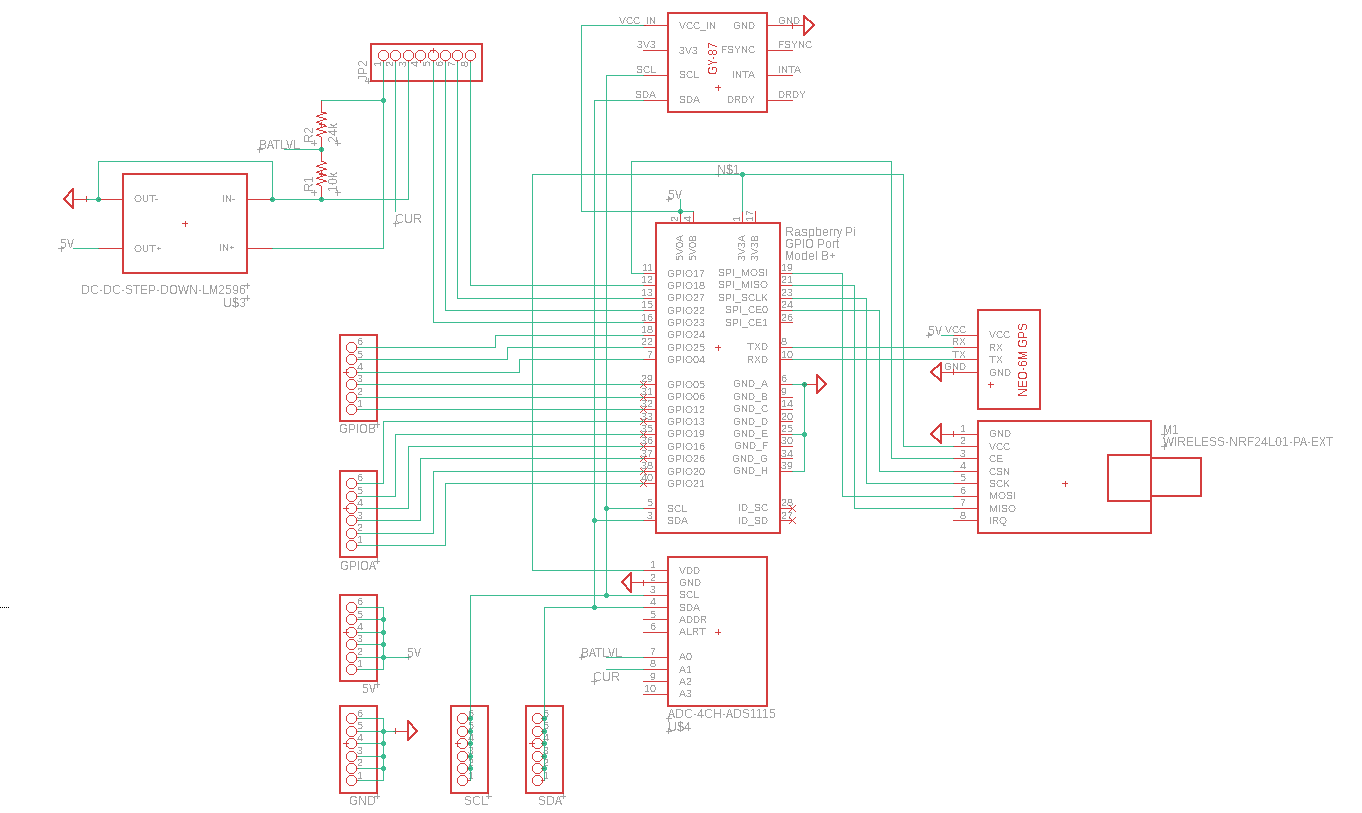
\includegraphics[scale=0.6]{images/fc_schematic.PNG}
    \caption{Schematic of the flight controller}
    \label{fig:fc_schematic}
\end{figure}
\begin{figure}[h]
    \centering
    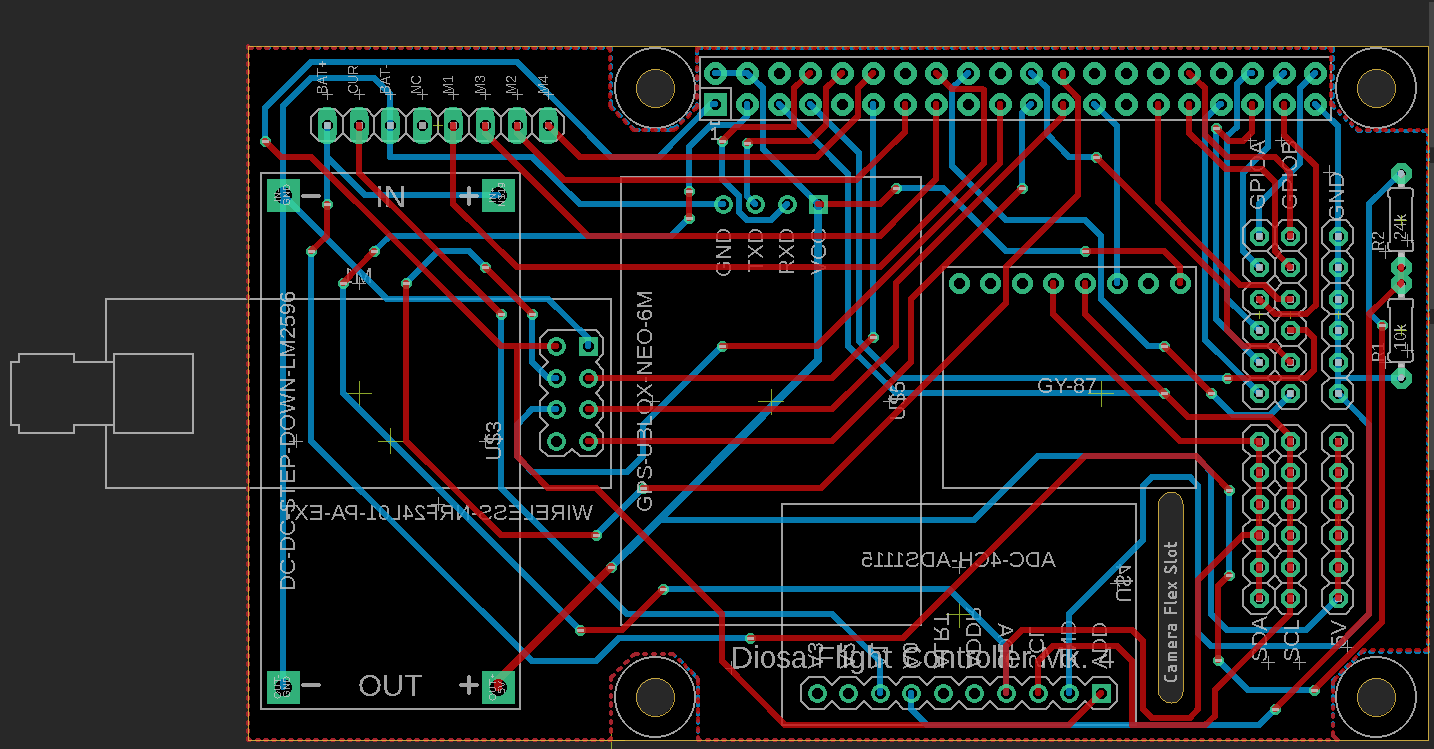
\includegraphics[scale=0.5]{images/fc_layout.PNG}
    \caption{Layout of the flight controller circuit board}
    \label{fig:fc_layout}
\end{figure}
\begin{figure}[h]
    \centering
    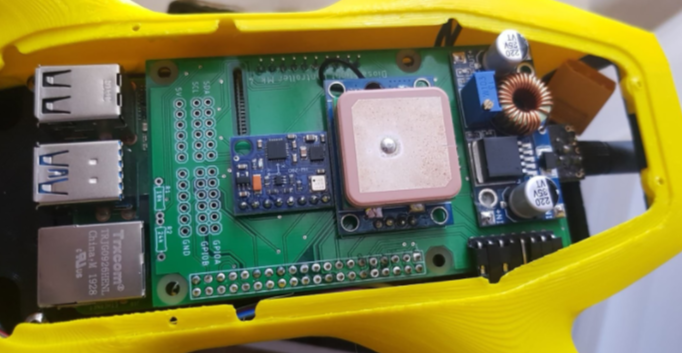
\includegraphics[scale=1]{images/fc_fab.PNG}
    \caption{Fabricated and assembled flight controller placed inside the Project Diosa chassis}
    \label{fig:fc_fab}
\end{figure}

\section{Base Station Design}
Though not quite the focus of the project as the base station may be redesigned as necessary, it was still important from a testing
standpoint to develop a base station that was mobile and could easily display data for on-the-field debugging. Figure \ref{fig:diosa_base_station}
shows the fully assembled base station. It features two analog joysticks for control over throttle, pitch, roll, and yaw. It also has four auxiliary
toggle switches that can be programmed on the flight controller. It is powered by a 2S lithium polymer battery. The base station also features
a 7inch touchscreen display though, for future developments, it might be noted that the display need not be touchscreen.

\begin{figure}[h]
    \centering
    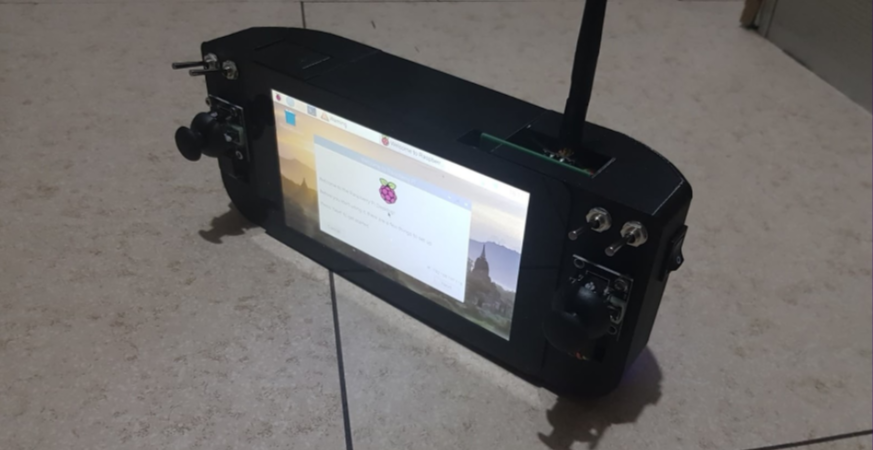
\includegraphics[scale=0.6]{images/diosa_base_station.PNG}
    \caption{Assembled mobile base station}
    \label{fig:diosa_base_station}
\end{figure}

\section{Relevant Testing}
\subsection{Communication and UAV Response Test}
During flight, it is important that communication between the UAV and the base station is kept. Thus, there is a need to verify that
packets sent to and from the UAV are consistent with packets sent from and to the base station.
Previously, the plan for testing the communications was to send incrementing values to the flight controller and compare the values
that the flight controller received against the values that the base station sent in order to see if there were any discrepancies
between the two. However, because the flight controller was programmed to send back an ACK packet to the base station in response to
received commands, it was deemed just as efficient to count how many ACks were returned in response to commands given. If an ACK isn't
received by the base station, we can assume that the previously sent packet was dropped. The target for this test is that there should
be no more than 5\% of packets lost.

\subsection{Stability Testing}
\begin{figure}[h]
    \centering
    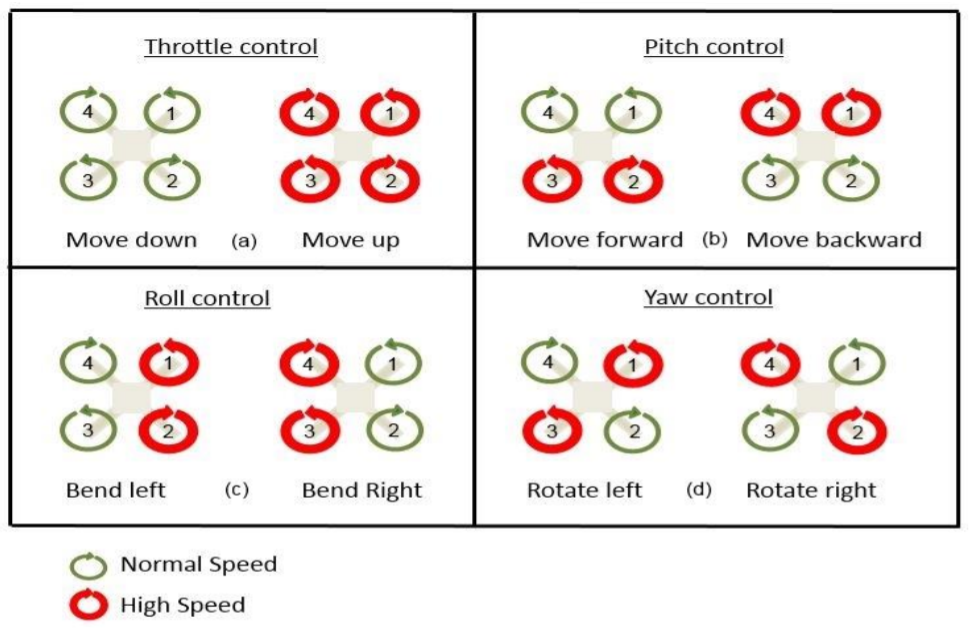
\includegraphics[scale=0.5]{images/motor_signals.PNG}
    \caption{Controlling the UAV \cite{fcDesign2019}}
    \label{fig:motor_signals}
\end{figure}
We may then move on to tuning and stability testing. As mentioned previously, test flights
were conducted and the PID coefficients were adjusted to obtain the values that produce the least amount of mean error in the
system. In order to fully test the flight performance, four tests were initially planned; the hover test, the pitch test, the roll test, and
the yaw test. The hover test supposedly establishes a baseline for the pitch, roll, and yaw tests. Further testing of the mentioned axes then
served to view how the axes would react while the other axes were held constant. One problem encountered, however, was the lack of air space where
one might safely and legally test a UAV. Another hurdle at the time of this project was the pandemic and the risks that came with venturing 
out into public spaces. Because of this, conducting the pitch, roll, and yaw tests (which required quite a bit of space) could not be done safely.
Upon further review\cite{zimmerman2016}, however, it was found that the hover test was enough for us to see how the PID controller would perform.
The hover test also did not require large spaces as the goal was to manually control the drone such that it hovered above one spot. 
During this test, we observed the error
responses for the roll, pitch, and yaw PID systems (recall roll, pitch, and yaw from the RRW and from figure \ref{fig:motor_signals}).
Error in the system was measured by taking the user commanded value of the parameter and subtracting from it the measured steady 
state value for the corresponding parameter from the IMU. An illustration of the experiment is shown by figure \ref{fig:error_diagram}.
\newline
\newline
The purpose of the \textbf{hover test} is to establish a baseline for the succeeding tests. In this test, the pilot
will attempt to make the UAV hover in place. While keeping the throttle at a constant value, the pilot will adjust pitch, roll, and yaw
in order to keep the UAV hovering in one spot. Measurement of the exact coordinates is not vital as what we are really looking for is
flight characteristics and whether or not the UAV can achieve stable flight.
\newline
\newline
Data over the course of the test was then compiled and the mean error was viewed over time. In this instance, system error 
is measured in degrees of rotation along a certain axis. Zimmerman's microcontroller based
flight controller has a mean error of 0.001\textdegree with a standard deviation of 0.4816\textdegree. These parameters were
treated as the baseline. Thus, the mean error of our end system should not exceed 0.001\textdegree and the standard deviation should 
not exceed 0.4816\textdegree. Should the parameter error responses not meet these conditions, the PID coefficients will be changed and the
tests will be repeated. If the conditions are met, the UAV is considered capable of stable flight. The results of these tests will be further
discussed in the Results and Analysis chapter.

\begin{figure}[h]
    \centering
    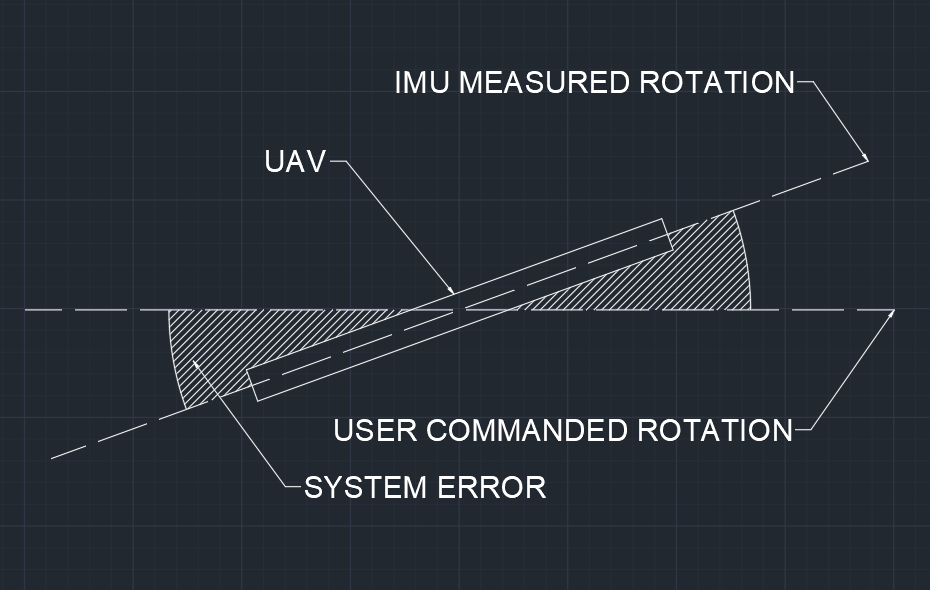
\includegraphics[scale=0.5]{images/error diagram.PNG}
    \caption{2-Dimensional Testing diagram}
    \label{fig:error_diagram}
\end{figure}

\chapter{Results and Analysis}
\section{Communication and UAV Response Test}
For the communications test, the packet loss was observed over the course of a minute after startup of the UAV. A summary of the results may
be view in figure \ref{fig:comms_plot}. Packet loss here is viewed in \% while time is in seconds. As can be seen from the plot, there is a huge
spike in packet loss right after the UAV starts up. There are also smaller spikes that occur within a few seconds of each other, though they aren't
quite as drastic. For the most part, however, packet loss remains below the targeted 5\% and seems to approach 1\%. Through multiple tests, 
the initial spike in packet loss can be seen as a constant occurrence. This could be attributed to connection errors upon startup. Further 
spikes in packet loss were attributed to noise in the system. It is important to note as well that direct line of sight between the base station 
and flight controller was maintained throughout the duration of the test. Based on the results of the test, we may conclude that communication
between the base station and flight controller is stable enough for the purposes of the project.
\begin{figure}[h]
    \centering
    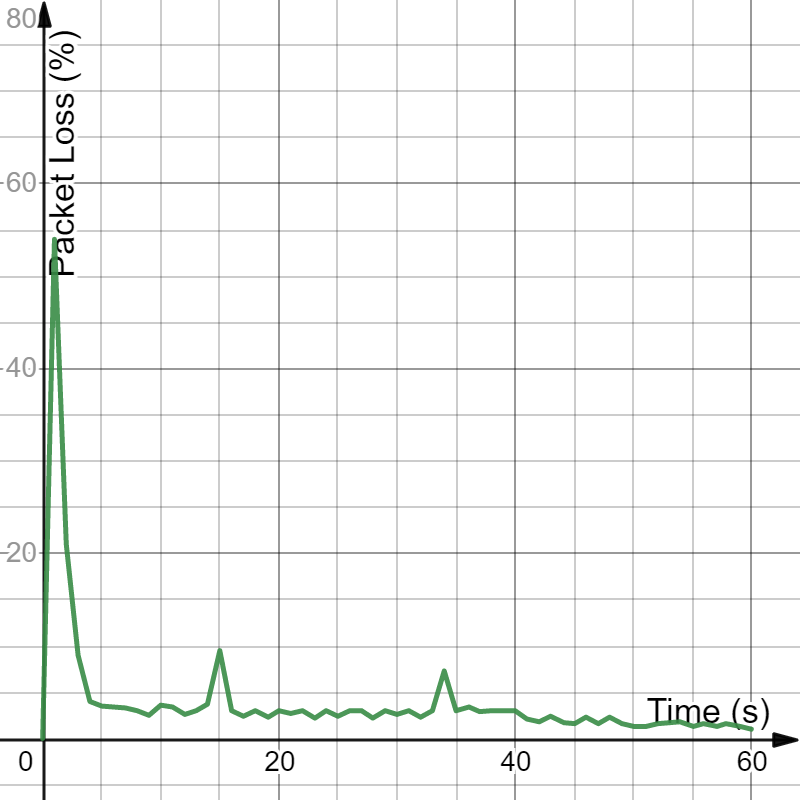
\includegraphics[scale=0.3]{images/comms_plot.png}
    \caption{Packet loss plot with respect to time}
    \label{fig:comms_plot}
\end{figure}
\section{Stability Testing}
Shown in figure \ref{fig:pid_plot} is a four second snippet of the control errors in response to the hover test. The blue, red, and green lines
are the plots for the pitch, roll, and yaw errors respectively. Taking the mean for each, the mean error for pitch is -0.0045\textdegree, the mean
error for roll is 0.01925\textdegree, and the mean error for yaw is 0.046\textdegree. Meanwhile, taking the standard deviation of each plot, we have
0.3981\textdegree, 0.2490\textdegree, and 0.4736\textdegree for pitch, roll, and yaw respectively. 
\newline
\newline
Recall that the target maximum absolute mean error
for any of the axes is 0.001\textdegree. Unfortunately, none of the control parameters were able to reach this goal. The current mean errors were
tested through various PID coefficients however these were the closest to the set goal. Failure to reach the goal is attributed to a number of factors.
The first one is differing systems. Zimmerman's implementation, which the goal was based on, ran C code on a microcontroller. Meanwhile, the system
used for this project runs on a much bigger and less efficient computer. Furthermore, the code is currently run on python3.7, which is much more
taxing and slower than its C and C++ counterparts. Second, upon closer inspection, the degree readings from the IMU and the analog sticks on the
base station could not reach an accuracy of 0.001\textdegree. Attempting to read that much accuracy from either part resulted in noise.
Fortunately, the errors are not so bad that the UAV is unable to perform flight. Possible fixes include coding in C++, which ROS' language agnosticism
allows, and implementing an IMU and analog stick + ADC that are more accurate and resistant to noise.
\newline
\newline
Lastly, recall that the target maximum standard deviation is 0.4816\textdegree. Fortunately, all of the control parameters were able to reach
the target, allowing us to at least hit one of our stable flight conditions. It might be noted that at 0.4736\textdegree, the yaw has the greatest
standard deviation among the three parameters. The same goes with the absolute mean error. This is attributed to the lack of multiple sensors to read
changes in yaw, which therefore results in greater inaccuracies. As mentioned earlier, we did implement an anti-drift algorithm for the yaw but
upon closer inspection and given enough time, it was found that the drift does still persist. This could mean that the calibration period was not
long enough to properly detect the drift rate. A possible fix to this would be to increase the calibration period. However, we then run into the
trouble of escalating the calibration period every time we detect drift. The better fix to this would be to employ more sensors that could aid in
the detection of changes in yaw, particularly a magnetometer.

\begin{figure}[h]
    \centering
    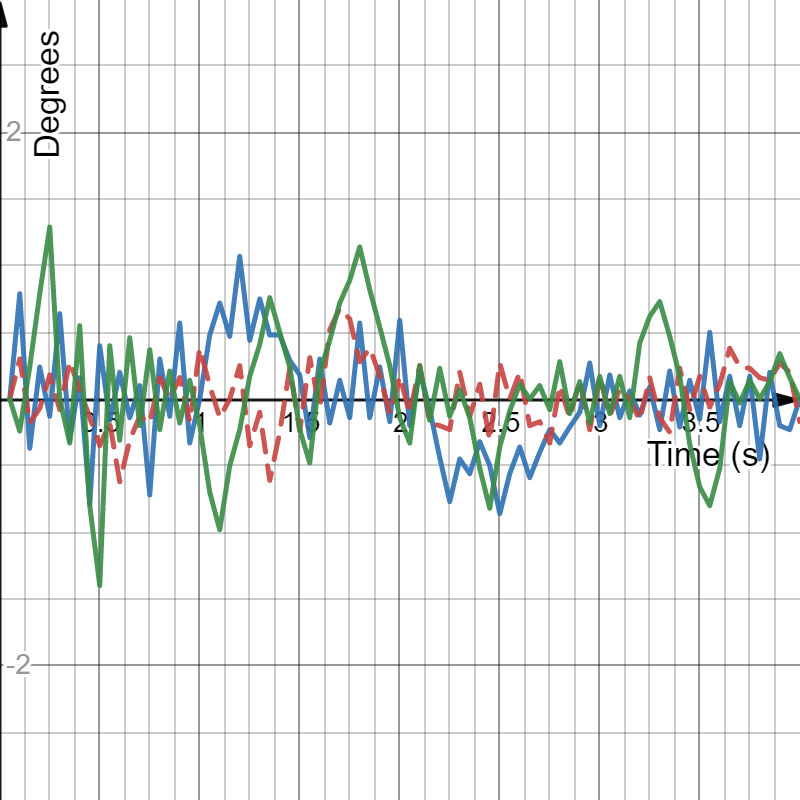
\includegraphics[scale=0.3]{images/pid_plot.png}
    \caption{Pitch (blue, solid), Roll (red, dotted), and Yaw (green, solid) control errors with respect to time in response to the hover test}
    \label{fig:pid_plot}
\end{figure}

\chapter{Conclusion}
The goal of this project was to see if it was possible to develop a flight controller system solely based on single board computers such as the
Raspberry Pi and without employing microcontrollers. Doing so gives the flight controller direct access to higher level functions and could serve
as a solid foundation for developments in unmanned aerial vehicle technology in the future. Through the implementation of various algorithms and
equations, we were able to develop a single-board computer based UAV with modular software and hardware. We were able to implement a robust communications
system that allows us to reliably send data to and from the flight controller. The PID control system, while not as stable nor accurate as what was
stipulated before, still allows us to fly the UAV with reasonable control.

\chapter{Recommendations for Future Work}
While the flight controller does afford us some degree of control, there are still obvious improvements that can be made. The first would be to
translate all of the code from python to c++. While python is powerful and versatile, it is more inefficient than its c++ counterpart. Inspection
of Raspberry Pi's CPU usage showed that during normal flight control operations, CPU usage stayed at a constant 97-100\%, leaving little room for
added operations. Another improvement would be to use a much more reliable and accurate IMU module. The GY-87 was used for this project due to its
availability in the local market. However, there are existing IMU modules that are similar to the GY-87 but are more recent. Lastly, the Raspberry Pi 4
was used for the project due to its availability and ease to prototype with. Employing more compact single-board computers such as the Raspberry Pi
compute module, which has the added benefit of being cheaper and more powerful, could pave the way for future developments in this line of flight controllers.

\chapter{Timeline}
\section{Gantt Chart}
\begin{figure}[h]
    \centering
    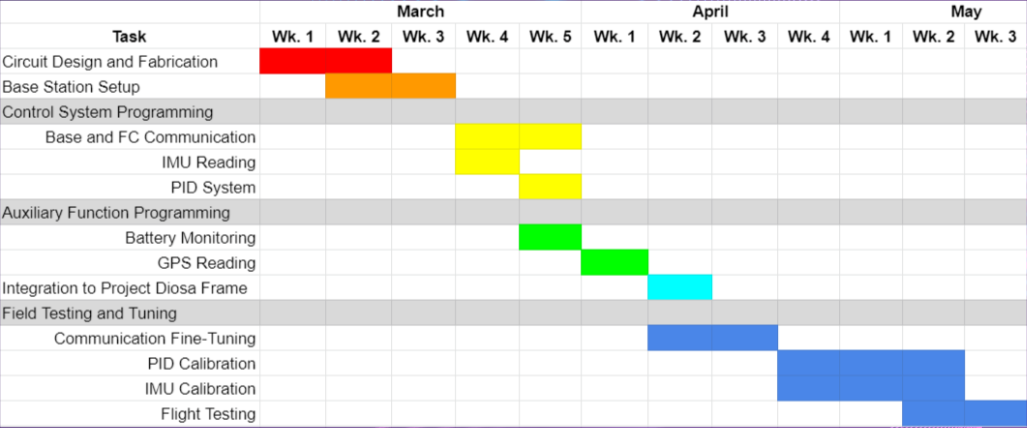
\includegraphics[scale=0.6]{images/gantt_chart.PNG}
    \caption{Project gantt chart}
    \label{fig:gantt_chart}
\end{figure}

\printbibliography[
heading=bibintoc,
title={Bibliography}
]

\end{document}

